\chapter{Conception}
\label{sec:Conception}

Building upon the insights from previous chapters regarding the pivotal role of haptic feedback, this chapter transitions from theoretical discussions to the practical implementation phase of our study. We have explored the rationale for incorporating haptic feedback, its intended applications, and the specific tools planned for use. Now, we move forward to actualize these concepts, beginning with a general use case diagram to visually represent system interactions. Following this, we will examine the visual aspects of our 3D interface and conclude by elucidating the underlying mechanisms that support our proposed solutions. This comprehensive approach ensures that our transition into the implementation phase is well-founded, aiming to enhance user experience through detailed planning and thoughtful design.

\section{General Use Case}
\label{sec:GeneralUseCase}

This section introduces the General Use Case diagram, which serves as a crucial visual tool depicting the dynamic interactions between users and the core functionalities planned for our \ac{VR} environment experiment. This diagram provides a comprehensive overview of the various scenarios and interactions that users may encounter, elucidating how they engage with the key features incorporated into the system.

\begin{figure}[ht]
\centering
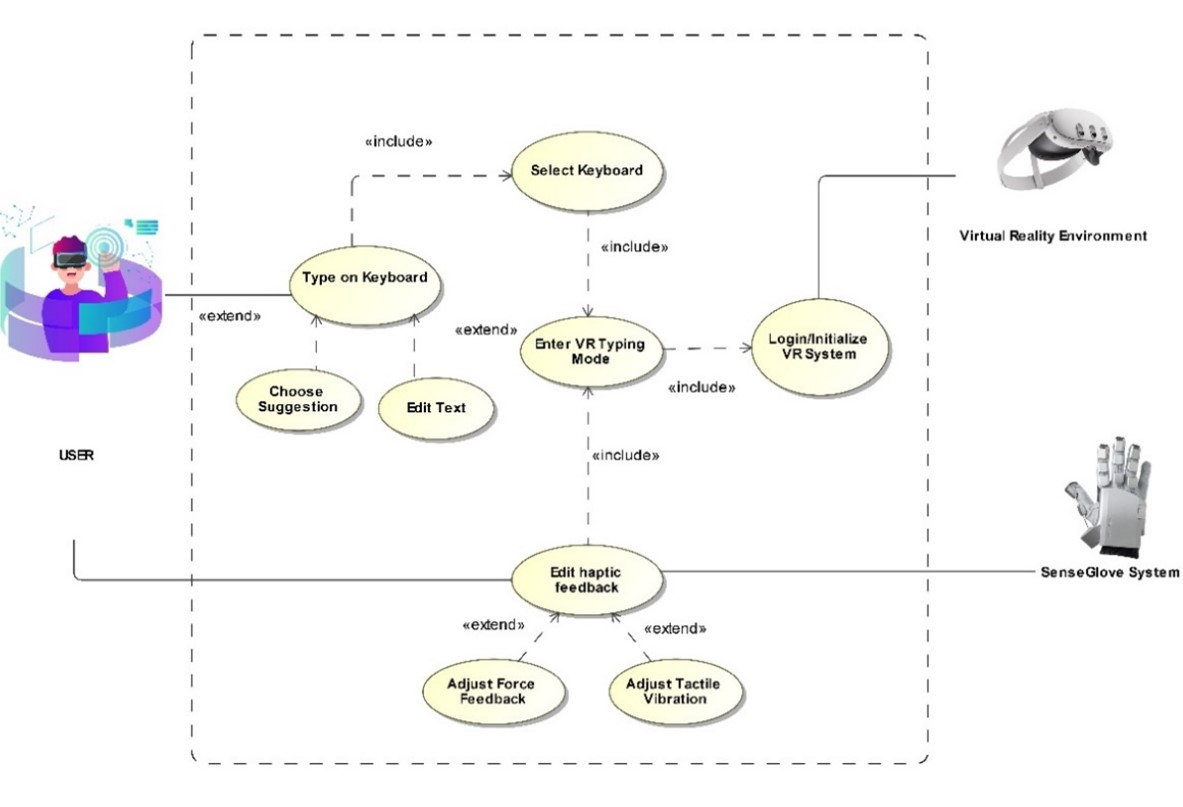
\includegraphics[width=0.8\textwidth]{Development/Picture1.jpg}
\caption{General Use Case Diagram for our experiment}
\label{fig:GeneralUseCaseDiagram} 
\end{figure}
\noindent Accompanying the diagram, Table~\ref{tab:GeneralUseCases} details the specific use cases, providing a structured description of each scenario within the \ac{VR} environment. This table categorizes user interactions, from initiation through various interaction phases, to modifications in settings, highlighting the system's response to each action.

\begin{table}[htbp]
\centering
\begin{tabular}{|p{4cm}|p{8cm}|}
\hline
\textbf{Use Case} & \textbf{Description} \\
\hline
Login/Initialize \ac{VR} System & To initiate the activity, the user is required to verify their identity, ensuring secure access to the virtual environment. \\
\hline
Enter \ac{VR} Typing Mode & Following successful login, the user transitions seamlessly into the immersive virtual typing environment. \\
\hline
Select Keyboard & The user selects the keyboard layout and settings to start typing, choosing from various available configurations. \\
\hline
Type on Keyboard & Interaction begins as the user types on the virtual keyboard, engaging with digital content creation. \\
\hline
Choose Suggestions & Users can select from contextually relevant suggestions provided by the system while typing, enhancing typing efficiency and accuracy. \\
\hline
Edit Text & Users have the flexibility to edit text at any point, with options to add, delete, or rearrange content as needed. \\
\hline
Edit Haptic Feedback & Users can enter a mode to customize the haptic feedback settings according to their personal preference. \\
\hline
Adjust \ac{FFB} & Users can fine-tune the intensity of \ac{FFB} to match their desired level of tactile response. \\
\hline
Adjust Tactile Vibration & The intensity of tactile vibrations can be adjusted, allowing users to tailor the haptic experience to their comfort and liking. \\
\hline
\end{tabular}
\caption{Descriptions of General Use Cases}
\label{tab:GeneralUseCases}
\end{table} 
\noindent Each use case outlines critical interactions within the system, ensuring that user needs and preferences are meticulously catered to, from system initiation to detailed personalization of the typing experience. This structured approach not only enhances user satisfaction but also fosters an intuitive and engaging interaction environment.
\clearpage
\section{Network Diagram}
\label{sec:NetworkDiagram}

Following the identification of the primary use cases, we now focus on examining the intercommunication among the key hardware components of our \ac{VR} environment setup. The network diagram presented in Figure~\ref{fig:NetworkDiagram} offers a detailed visual representation of the interaction among these components, which include advanced haptic gloves, the Execution Environment, the local subnet, and the \ac{HMD}. This diagram is essential for understanding how data flows within our system and how components are interconnected to support seamless user interactions.

\begin{figure}[htbp]
\centering
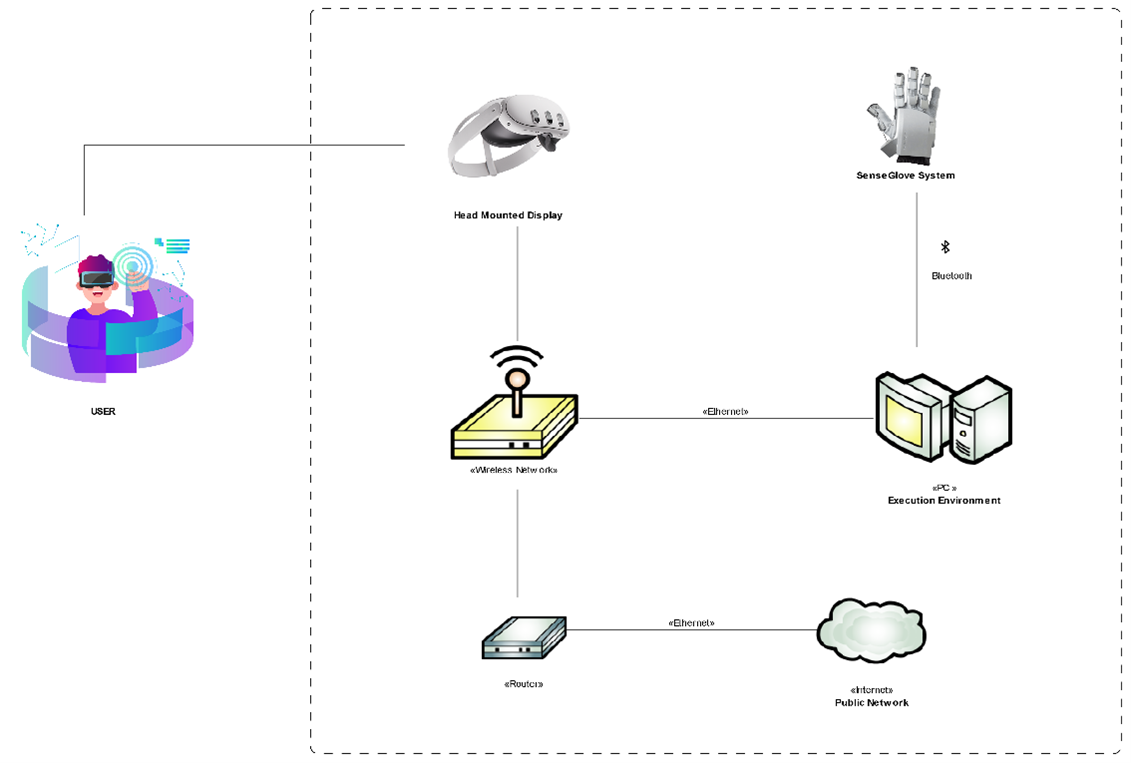
\includegraphics[width=1\textwidth]{Development/networkDiagram.png}
    \captionsetup{justification=centering}

\caption{Network Diagram showing the interconnectivity of system components.}
\label{fig:NetworkDiagram}
\end{figure}

\clearpage

\begin{table}[htbp]
\centering
\begin{tabular}{|p{3cm}|p{9cm}|}
\hline
\textbf{Hardware} & \textbf{Description} \\
\hline
SenseGlove Nova & The SenseGlove Nova transmits sensory data to the Execution Environment via Bluetooth. It can also establish a direct connection to the \ac{HMD} when required. \\
\hline
Wireless Network & Communication between the \ac{HMD} and the Execution Environment is facilitated through Air Link, a high-performance wireless connection that supports real-time data exchange. \\
\hline
Execution Environment & All scenario executions occur locally within this environment, employing Bluetooth as the primary communication protocol to ensure rapid and secure data transfer. \\
\hline
Router & The router plays a pivotal role in managing communications between the \ac{HMD}, Execution Environment, and the public internet, ensuring robust and reliable connectivity. \\
\hline
Head-Mounted Device (\ac{HMD}) & The \ac{HMD} communicates with the Execution Environment using the TCP protocol to facilitate seamless access and synchronization with the public internet. \\
\hline
\end{tabular}
\caption{Descriptions of the Network Diagram Components}
\label{tab:NetworkDiagram}
\end{table}
\noindent
This network setup is designed to optimize the flow of information and control signals across different components of the system, ensuring that the \ac{VR} environment operates smoothly and efficiently. The integration of these components via robust communication protocols and network connections is critical for delivering a responsive and immersive user experience, thereby enhancing both the realism and functionality of the virtual environment.

\section{Virtual Keyboard’s Conception}
\label{sec:Virtual Keyboard Conception}
While smartphones have become the most used hardware in the market, surpassing other devices \cite{Laricchia2024}, they still rely on fundamental components common to many hardware devices. For instance, consider the conventional structure of a keyboard, which is an integral part of many devices, not just computers but also smartphones in the form of digital keyboards.\\ \\
The keyboard comprises two primary components: the keys and the substrate. The substrate is a planar surface responsible for housing and supporting the keys. In the context of a smartphone, the ‘keys’ are the touch-responsive elements displayed on the screen, and the ‘substrate’ is the underlying software framework that captures and interprets key presses \cite{Staff2022}. Given user familiarity with the established paradigm of smartphone keyboard architecture, the design of the keyboard will conform to this norm. Consequently, emphasis will primarily be directed toward the clarification and optimization of the aforementioned two components.\\ \\
Hence, our goal is to replicate the smartphone keyboard in a \ac{VR} environment. The following sections delve into the intricacies of the keyboard design slated for use in the forthcoming immersive experience.

\subsection{Conceptualization of the Board}

To make a virtual keyboard look and act real, attention to detail is crucial. By replicating as many features as possible, the virtual version can seem more genuine. A study \cite{Ying2021} investigated the impact of QWERTY and T9 \cite{T9} input methods on smartphone text input across various sizes (4.7 inches, 5 inches, and 5.5 inches). Findings indicate that QWERTY is more effective for two-thumb input, and T9 for one-thumb input, with two-thumb entry providing an overall superior user experience. Optimal performance was observed with QWERTY and T9 on a 5-inch smartphone and QWERTY on a 5.5-inch smartphone.

\begin{figure}[h!]
    \centering
    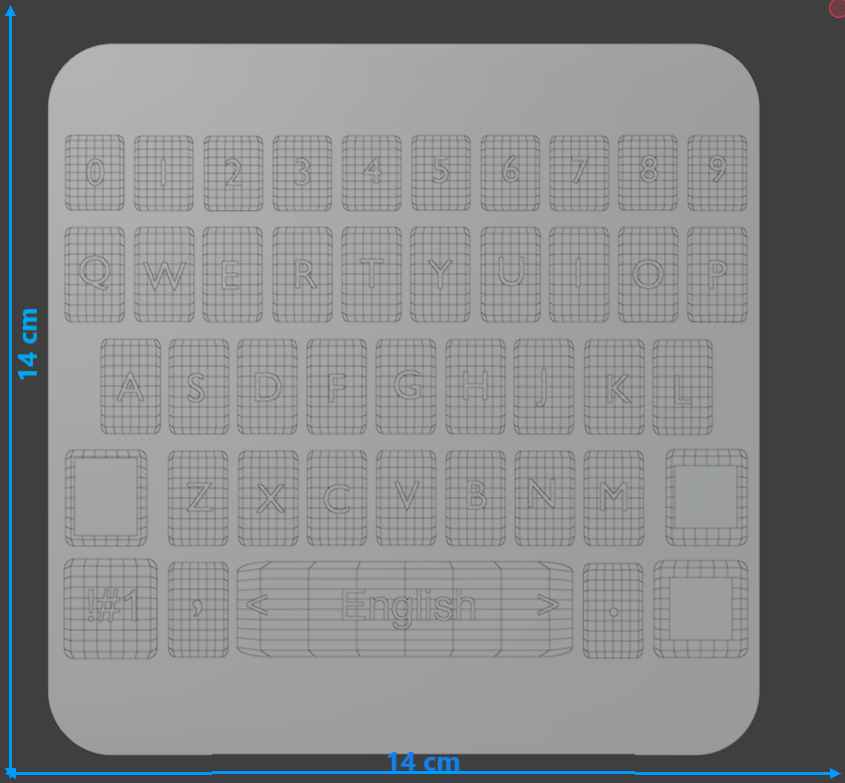
\includegraphics[width=0.7\linewidth]{Development/keyboard_size.png}
    \caption{Schematic representation of the virtual keyboard layout used for testing QWERTY input methods, displayed in Blender viewport shading (Solid Display).}
    \label{fig:keyboard_sin}
\end{figure}
\noindent
In addition to keyboard size, the most commonly used colors for smartphone keyboards are black, gray, and white. This is supported by the popularity of black as a phone color and the prevalence of these colors in top Android keyboards like Fleksy, Gboard, and SwiftKey \cite{Muelaner2023}. These colors are likely chosen for their neutrality, which allows them to blend well with various phone themes and user preferences.\\ \\

\begin{figure}[h!]
    \centering
    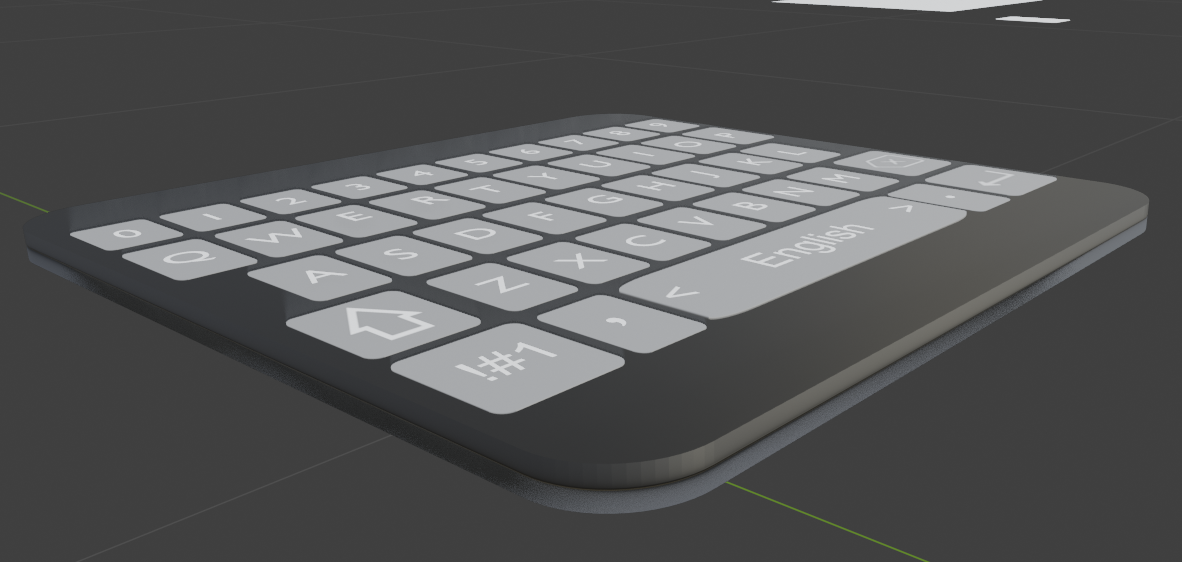
\includegraphics[width=0.7\linewidth]{Development/keybordViewPort.PNG}
    \caption{Schematic representation of the virtual keyboard layout used for testing QWERTY input methods, displayed in Blender viewport shading (Material Display). }
    \label{fig:keyboard_sin}
\end{figure} \noindent
To enhance the portability of our keyboard, integrating hand support is imperative, aiming to emulate the familiar grip of a smartphone. This augmentation contributes to a heightened sense of realism and immersion in \ac{VR} experiences, allowing users to interact with the keyboard in a manner akin to physical settings, even while wearing gloves. Moreover, ensuring universal comfort necessitates careful consideration of users' hand dimensions. According to the National Aeronautics and Space Administration (NASA), the average hand length for males is 7.6 inches, with a breadth of 3.5 inches and a circumference of 8.6 inches. Correspondingly, for females, these dimensions are 6.8 inches, 3.1 inches, and 7.0 inches, respectively. Incorporating this data allows us to ensure that the thumb can comfortably reach the edge of the keyboard when the user enters the typing mode, ensuring a user-friendly and universally comfortable device \cite{nasa_anthropometry,nasa_hand_dimensions,nasa_performance}.

\subsection{Key Conception for the Keyboard}

In our pursuit to optimize the \ac{VR} keyboard and replicate the efficiency of physical typing, we propose a distinctive proportion mechanism aimed at minimizing typing errors. This mechanism operates by identifying the key with the largest contact area with the virtual finger. To streamline this process, we advocate for the division of each virtual key into multiple sections.\\ \\
To implement this division, we suggest employing a grid-based method. Each virtual key's surface is subdivided into cells of equal size, forming a grid. The dimensions of this grid are determined by the average size of the virtual fingertip and the size of the virtual key. For instance, if both the virtual key and the average virtual fingertip measure 10 mm x 10 mm, we could opt for a 3x3 or 8x10 grid configuration. \\ \\

\begin{figure}[h!]
    \centering
    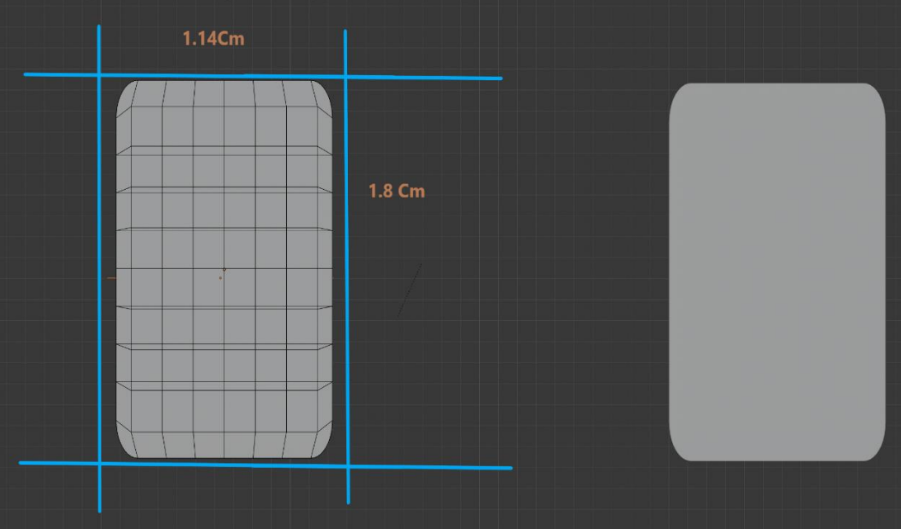
\includegraphics[width=1\linewidth]{Development/keyboard_image2.PNG}
    \caption{Schematic representation of the virtual key layout used for testing QW-
ERTY input methods, displayed in Blender viewport shading (Solid Display)}
    \label{fig:enter-label}
\end{figure}
\noindent 
The subsequent step involves scrutinizing each cell within the grid to assess the degree of contact with the virtual finger. This assessment is facilitated by incorporating a texture on the surface of the thumb finger of the virtual hand model, as provided by the SenseGlove Nova SDK. \\ \\
To enhance the user experience, we propose integrating an animation feature. The shape of the virtual key during interaction will mimic the shape it takes when pressed on a smartphone. A pop-up animation will accompany this interaction, visually indicating the pressed key. When designing virtual keyboards, particularly the size of the keys, it's essential to balance ergonomics with functionality to enhance user experience and performance. Research indicates that key size can significantly affect typing speed, accuracy, and overall comfort. According to a study \cite{Kim2013}, key sizes on touch screen virtual keyboards influence productivity, usability, and typing biomechanics, suggesting that virtual keyboards with a key size less than 16 mm may slow typing speed and increase wrist extension, highlighting the importance of optimizing key size for user comfort and efficiency. Another study \cite{Productivity2014} proved that virtual keyboards with key sizes smaller than recommended (18 to 20 mm for notebook and desktop keyboards) can lead to slower typing speeds, higher muscle activity, and greater wrist extension, indicating potential discomfort and reduced productivity. Keyboards with 13x13 mm keys, for example, resulted in a 15\% slower typing speed and higher static shoulder muscle activity compared to larger key sizes.\\ \\
For a \ac{VR} smartphone keyboard, choosing the right texture for the keys is essential to enhance realism and user experience. The texture should provide visual cues that simulate the feel of a real keyboard. Research in human-computer interaction (HCI) \cite{Fitts2004} has shown that reducing glare and reflections on surfaces can improve visibility and reduce eye strain. A Dark texture on the \ac{VR} keyboard keys can help achieve these goals, making it easier for users to see and interact with the keyboard.

\section{Dynamic Virtual keyboard Interactions}

\subsection{Key Press Animation Feedback}
For key press animation, the goal is to provide immediate feedback to the user, indicating that their input has been recognized. This type of animation falls under the category of micro-interactions. These animations are crucial in making interactions feel more tangible and responsive \cite{Hannah2021}. Therefore, a 0.2-second animation at 30 frames per second, resulting in 6 frames, would be consistent with these principles, offering a quick and responsive feedback loop that enhances the user experience without overwhelming the user with unnecessary motion or delay.\\ \\
In our project, the scale values were adjusted during the animation. The X and Y components were each increased by approximately 11\%, while the Z component was increased by approximately 4\%. These adjustments were calculated to provide a noticeable yet subtle feedback effect, aligning with the principles of effective micro-interactions and ensuring a smooth, responsive user experience. We found that this scale percentage is the optimal size to avoid key collision during scaling, ensuring that the keys remain distinct and accessible during the animation. 
 \begin{figure}[h!]
\centering
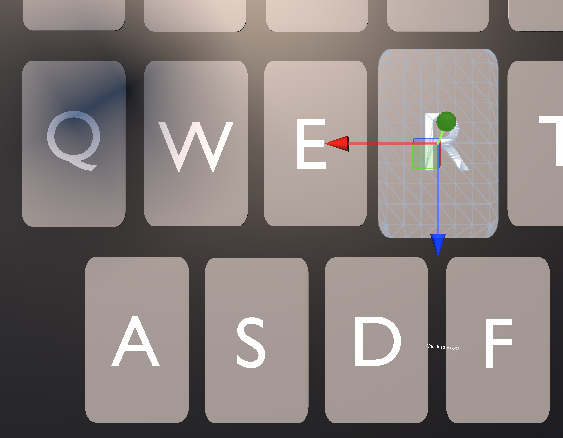
\includegraphics[width=0.8\textwidth]{Development/key_AfterAnimation.PNG} 
\caption{Key Appearance After Animation}
\end{figure}

\noindent
\\\\                
\noindent
\\\\  \noindent
\\\\  \noindent
\\\\  \noindent


\subsection{Hover Effect Implementation}

In virtual reality (VR) environments, providing immediate visual feedback to users significantly enhances their interaction experience, improving both accuracy and comfort. One critical aspect of this feedback mechanism is the hover effect, which visually highlights key parts as users move their fingers over them. This section explains the logic behind the hover effect implementation in the VR keyboard, including the dynamic color changes of the key parts.

\subsubsection{Detection of Hovered Key Parts}

The hover effect is implemented by continuously monitoring the position of the user's thumb in the VR environment. A virtual bounding box is defined around the thumb, and this box is used to detect any interaction with the virtual keyboard key parts.

\subsubsection{Raycasting Technique}

To determine which key parts are being hovered over, a technique called raycasting is used. This involves projecting a virtual box around the thumb's position and checking for intersections with the key parts on the virtual keyboard. The system identifies which key parts are within this box, indicating that they are being hovered over by the user's thumb.

\subsubsection{Visual Feedback Mechanism}

Once a key part is detected as being hovered over, the system provides immediate visual feedback by changing the appearance of the key part. This visual change primarily involves altering the color of the key part. The color transition is determined based on a predefined start color and end color, and the specific weight assigned to each key part. The weight represents the degree of interaction or importance of the key part, allowing for a smooth gradient transition between the start and end colors \cite{douglas1999impact} .

\subsubsection{Handling Multiple Key Parts}

The system keeps track of the key parts that were previously hovered over. If the thumb moves away from a key part, the visual feedback for that key part is reset to its original state. This ensures that only the currently hovered key parts are visually highlighted, providing real-time feedback as the user moves their thumb across the virtual keyboard.

\subsubsection{Interaction States}

The hover effect is closely integrated with the overall interaction states of the virtual keyboard. When no key part is actively being pressed, the system focuses on detecting and highlighting the key parts being hovered over. If a key part is pressed, the hover detection is temporarily paused to prevent conflicts between hover and press feedback.

\subsubsection{Dynamic Color Adjustment}

The system dynamically adjusts the color of the key parts based on the user's actions. When a key part is hovered over, its color changes according to a calculated weight. The weight determines the blend between the start and end colors, using a linear interpolation technique to create a smooth transition. This provides immediate and clear visual feedback, enhancing the user's interaction experience. When the thumb moves away, the key part's color is reset to its original state, ensuring that the visual feedback accurately represents the current interaction state \cite{bolt1980put}.

\subsubsection{User Experience Enhancement}

By providing immediate and clear visual feedback through the hover effect, including dynamic color changes, the system enhances the user's typing experience in the VR environment. Users can easily see which key parts they are about to press, reducing errors and increasing typing efficiency. This real-time feedback is crucial for creating a more intuitive and engaging virtual interaction \cite{norman2013design}.

\subsection{Key Press Sound Feedback} 

In our project, we aimed to generate unique audio feedback for each key press on a virtual keyboard. The process involved modifying the pitch of a base click sound to create distinct auditory signals for each key, ensuring that each key press has a unique sound effect. This approach enhances the user experience by providing clear and immediate auditory feedback, aligning with the principles of effective micro-interactions. We utilized the \texttt{pydub} library for audio processing \cite{pydub}, which was responsible for loading, modifying, and exporting audio files.

\subsubsection*{1. Pitch Modification}

Pitch modification refers to changing the frequency of an audio signal to alter its pitch without changing its duration \cite{smith1999}. This is a crucial technique in audio processing used to create variations in sound.\\ \\
\noindent
The core principle behind generating unique sounds for each key is pitch shifting. Pitch shifting involves changing the frequency of an audio signal without altering its duration. Mathematically, this is achieved by altering the sample rate of the audio signal.
The relationship between the original frequency (\( f \)) and the modified frequency (\( f' \)) when shifting the pitch by \( s \) semitones is given by:
\begin{equation}
f' = f \cdot 2^{\frac{s}{12}}
\end{equation}


where:
\begin{itemize}
  \item \( f \) is the original frequency,
  \item \( f' \) is the new frequency after pitch shifting,
  \item \( s \) is the number of semitones by which the pitch is shifted.
\end{itemize}
\begin{figure}[h!]
    \centering
    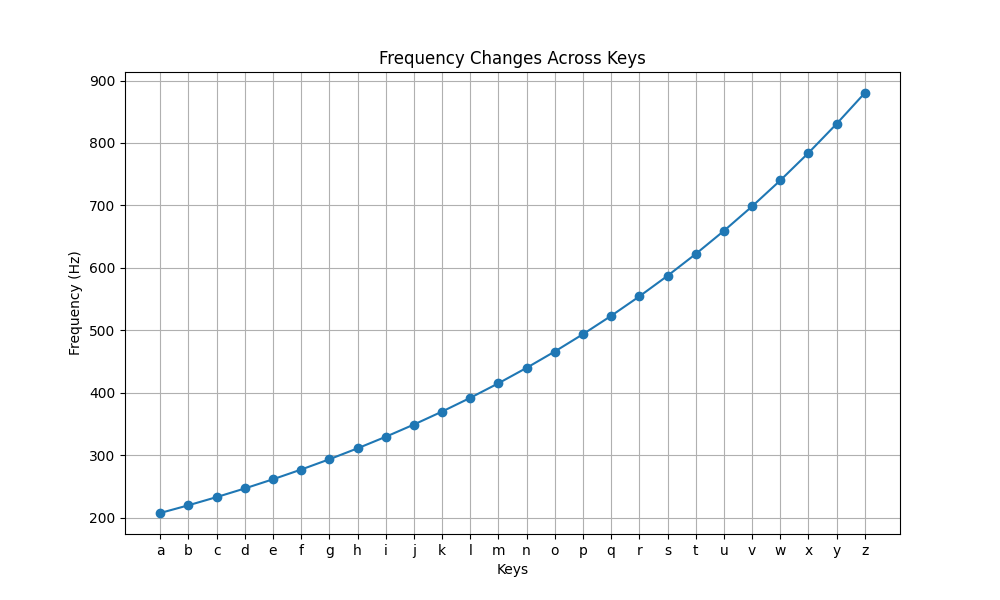
\includegraphics[width=0.8\linewidth]{Development/frequency_changes.png}
    \caption{Frequency changes across keys from 'a' to 'z'.}
    \label{fig:keyboard_sin}
\end{figure} \noindent
\subsubsection*{2. Sample Rate Adjustment}

Sample rate adjustment is the process of changing the sampling rate of an audio signal to alter its pitch. By modifying the sample rate, the pitch of the sound can be raised or lowered while keeping the duration constant \cite{jones2003}. \\ \\
\noindent
To implement this pitch shift, we adjust the sample rate of the audio signal. If the original sample rate is \( R \), the new sample rate \( R' \) after shifting the pitch by \( s \) semitones can be calculated as:
\begin{equation}
R' = R \cdot 2^{\frac{s}{12}}
\end{equation}
By resampling the audio signal to this new sample rate and then adjusting it back to the original sample rate, we effectively change the pitch while maintaining the duration of the audio. \\ \\
The sample rate adjustment is executed within the \texttt{change\_pitch} function. Initially, we calculate the new frame rate (\( R' \)) based on the desired pitch shift in semitones. We use the \texttt{\_spawn} method from the \texttt{pydub} library to create a new \texttt{AudioSegment} with the modified frame rate, which changes the pitch of the sound. Finally, we reset the frame rate back to the original to ensure the duration remains unchanged, thereby achieving the desired pitch modification.\\ \\
\noindent
\begin{figure}[h!]
\centering
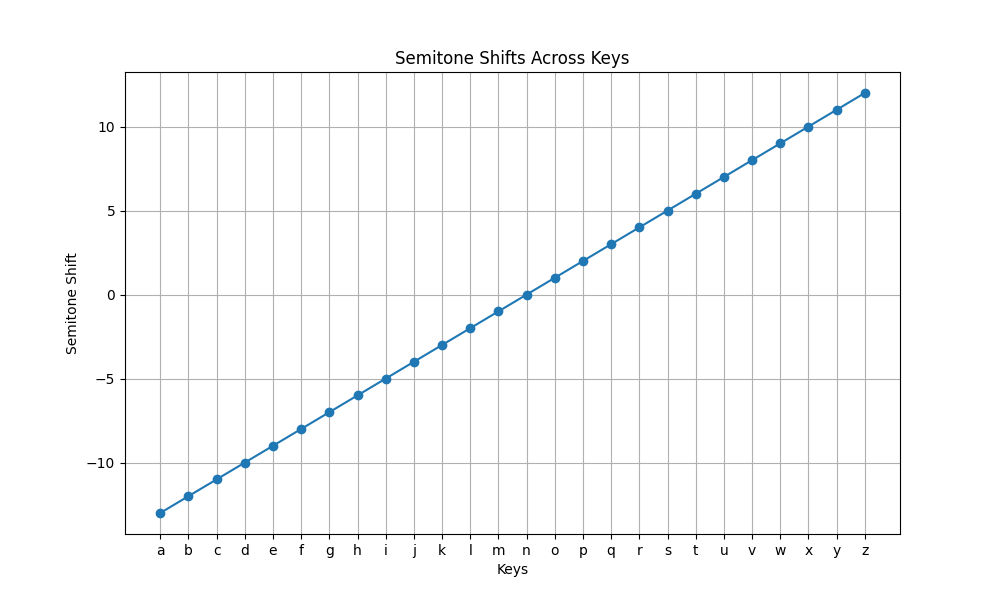
\includegraphics[width=0.8\textwidth]{Development/semitone_shifts.png}
\caption{Semitone shifts across keys from 'a' to 'z'.}
\end{figure} 




\subsubsection*{3. Application to Key Press Sounds}
For our virtual keyboard, we needed a unique pitch for each letter key (from 'a' to 'z'). We assigned a specific number of semitones to each key based on its position in the alphabet. The assignment is defined as follows:
\begin{equation}
s_i = i - 13
\end{equation}

where:
\begin{itemize}
  \item \( s_i \) is the pitch shift for the \( i \)-th letter,
  \item \( i \) is the index of the letter in the alphabet (0 for 'a', 25 for 'z').
\end{itemize}

\begin{figure}[h!]
\centering
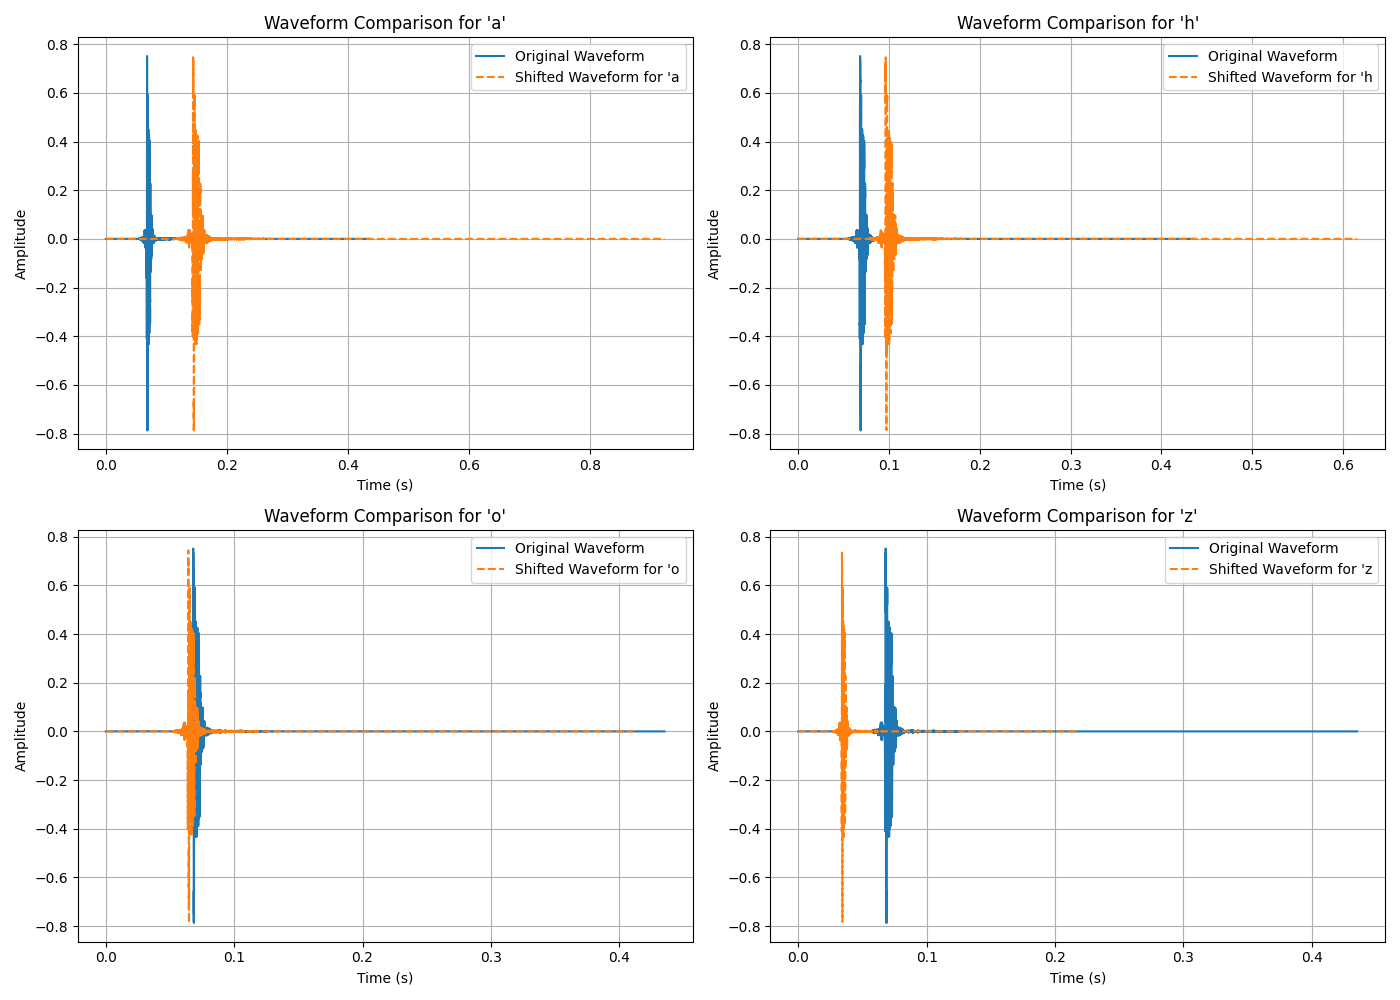
\includegraphics[width=0.8\textwidth]{Development/waveform_comparison_combined.png}
\caption{Waveform comparison of original and shifted sounds .}
\end{figure} 
\noindent \\\\\ \\ \\ 
This results in a pitch shift range from -13 semitones for 'a' to +12 semitones for 'z'.
By applying these mathematical principles of pitch shifting and sample rate adjustment, we generated distinct and responsive audio feedback for each key on a virtual keyboard. This method enhances the user experience by providing immediate and clear auditory confirmation of each key press, aligning with the principles of effective micro-interactions.

\subsection{Key Weight Calculation}
In the virtual keyboard simulation developed , we quantify the tactile feedback and the accuracy of the desired typed keys through a calculated "weight" assigned to each key and its respective parts. This weight metric plays a crucial role in simulating dynamic responses typical of physical keyboard interactions, which is essential for enhancing the accuracy of typing within the virtual environment. The need for such a simulation arises from the inherent discrepancies in the data frequencies between the frame rate of the virtual environment and the tracking system used for modeling hand movements. By synchronizing these elements through calculated key weights, we ensure that the user's interactions with the virtual keyboard are both intuitive and responsive, closely mimicking real-world typing experiences.


\subsubsection*{1. Key Part Weight Calculation}
The weight of each key part is determined based on its designated role and position within the key layout. For edge key parts, which are less frequently engaged during typing, a constant base weight is assigned, ensuring a uniform weight distribution for less significant key parts and is given by:
\begin{equation}
W_{\text{base}} = 0.1 \quad \text{(as an example value)}
\end{equation}
For central and more interactive key parts, the weight is dynamically calculated based on the key part's Cartesian coordinates on the keyboard grid. This method emphasizes the importance of centrally-located key parts:
\begin{equation}
W(x, y) = \frac{1}{\sqrt{(x - x_{\text{center}})^2 + (y - y_{\text{center}})^2 + 1}}
\end{equation}
where $x_{\text{center}}$ and $y_{\text{center}}$ represent the coordinates of the central key part of the keyboard, and the addition of 1 in the denominator prevents division by zero, ensuring that central key parts have the highest weights.

\subsubsection*{2. Overall Key Weight Calculation}
The total weight of a key at any moment is the sum of the weights of all its collided key parts. This sum is calculated periodically to determine the overall weight of the key:
\begin{equation}
W_{\text{key}} = \sum_{i=1}^{n} W_i
\end{equation}
where $W_i$ is the weight of the $i$-th collided key part. This cumulative weight is then used to identify the active key, which is the key with the highest total weight among all keys engaged at that instance.\\ \\
This approach models real-world typing by dynamically adjusting key sensitivity based on typical finger movements and interactions, thereby simulating an intuitive and realistic typing experience. The mathematical model ensures that the most probable key press is detected based on tactile feedback, which is crucial for providing accurate and responsive keyboard simulations.

\subsection*{3. Process Overview}
\begin{enumerate}
    \item \textbf{Collision Detection:} Each key part uses Unity's physics engine to detect collisions.
    \item \textbf{Event Notification:} Collisions trigger events that notify the parent key of the key part's status.
       \item \textbf{Register collided key:}
    The key notifies the keyboard upon activation and registers itself within the keyboard.
       
    \item \textbf{Weight Calculation:} The keyboard periodically checks all activated keys, aggregating the weights from their active key parts to calculate their total weights. It then identifies the key with the highest total weight
    
    \item \textbf{Key Press Detection:} A key is considered pressed if its aggregated weight is the highest among all keys.
    \item \textbf{Key Typed:} The determination of a key press is finalized when all collisions have ceased, particularly as the user lifts their finger from the key.
\end{enumerate}




















